% !TeX root = ../main.tex

\chapter{插图和表格}

\section{三线表}

三线表是《撰写手册》推荐使用的格式,如表~\ref{tab:exampletable}。

\begin{table}
  \centering
  \caption{表号和表题在表的正上方}
%  \bicaption{表号和表题在表的正上方}{Sample table 1}
  \label{tab:exampletable}
  \begin{tabular}{cl}
    \toprule
    类型   & 描述                                       \\
    \midrule
    挂线表 & 挂线表也称系统表、组织表,用于表现系统结构 \\
    无线表 & 无线表一般用于设备配置单、技术参数列表等   \\
    卡线表 & 卡线表有完全表,不完全表和三线表三种       \\
    \bottomrule
  \end{tabular}
\end{table}

\begin{table}[h] %voc table result
	\centering
	\caption{十分复杂的表格}
	\begin{tabular}{*{5}{c}}
		\toprule
		区域 & \tabincell{c}{外侧核热功率\\(MW)} & \tabincell{c}{内侧核热功率\\(MW)} & 结构 & \tabincell{c}{结构核热功率\\(MW)} \\
		\midrule
		第一壁涂层 & 20.0 & 13.4 & \multirow{2}{*}{第一壁} & \multirow{2}{*}{151.7} \\
		第一壁结构层 & 70.2 & 48.1 & ~ & ~ \\
		\midrule
		Be-1区 & 37.9 & 26.5 & \multirow{8}{*}{氚增殖区} & \multirow{8}{*}{970.2} \\ 
		Li$ _{\text{4}} $SiO$ _{\text{4}} $-1区 & 126.7 & 86.8 & ~ & ~ \\
		Be-2区 & 133.6 & 94.1 & ~ & ~ \\
		Li$ _{\text{4}} $SiO$ _{\text{4}} $-2区 & 134.4 & 96.2 & ~ & ~ \\
		Be-3区 & 68.6 & 49.7 & ~ & ~ \\
		Li$ _{\text{4}} $SiO$ _{\text{4}} $-3区 & 49.6 & 37.2 & ~ & ~ \\
		Be-4区 & 9.2 & 7.0 & ~ & ~ \\
		增殖区后支撑 & 7.1 & 5.5 & ~ & ~ \\
		\midrule
		屏蔽区(水) & 6.8 & 5.4 & \multirow{2}{*}{屏蔽区} & \multirow{2}{*}{18.2} \\
		屏蔽区(钢) & 3.3 & 2.7 & ~ & ~ \\
		\midrule
		总计 & 667.5 & 472.6 & - & 1140.1 \\
		\bottomrule
	\end{tabular}
	\label{nucheat_tot}
\end{table}

\begin{table}
	\centering
	\caption{从csv文件中导入表格}
	\begin{adjustbox}{max width=\linewidth}
	\csvautobooktabular{tables/asterids.csv}
	\end{adjustbox}
	\label{tab:asterid}
\end{table}

如果有表注,推荐使用 \pkg{threeparttable}。这样可以与表格对齐,满足部分评审老师的要求。

\begin{table}
  \centering
  \begin{threeparttable}
    \caption{带表注的表格}
%    \bicaption{带表注的表格}{Sample table 2}
    \label{tab:tablewithnotes}
    \begin{tabular}{cl}
      \toprule
      类型   & 描述                                       \\
      \midrule
      挂线表 & 挂线表也称系统表、组织表,用于表现系统结构 \\
      无线表 & 无线表一般用于设备配置单、技术参数列表等   \\
      卡线表 & 卡线表有完全表,不完全表和三线表三种       \\
      \bottomrule
    \end{tabular}
    \begin{tablenotes}[flushleft]
      \item 注:表注分两种,第一种是对全表的注释,用不加阿拉伯数字排在表的下边,
      前面加“注:”;第二种是和表内的某处文字或数字相呼应的注,
      在表里面用带圈的阿拉伯数字在右上角标出,然后在表下面用同样的圈码注出来
    \end{tablenotes}
  \end{threeparttable}
\end{table}

编制表格应简单明了,表达一致,明晰易懂,表文呼应、内容一致。
排版时表格字号略小,或变换字体,尽量不分页,尽量不跨节。
表格太大需要转页时,需要在续表上方注明“续表”,表头页应重复排出。



\section{插图}

有的同学可能听说“\LaTeX{} 只能使用 eps 格式的图片”,甚至把 jpg 格式转为 eps。
事实上,这种做法已经过时。
而且每次编译时都要要调用外部工具解析 eps,导致降低编译速度。
所以我们推荐矢量图直接使用 pdf 格式,位图使用 jpeg 或 png 格式。

\begin{figure}[h]
  \centering
  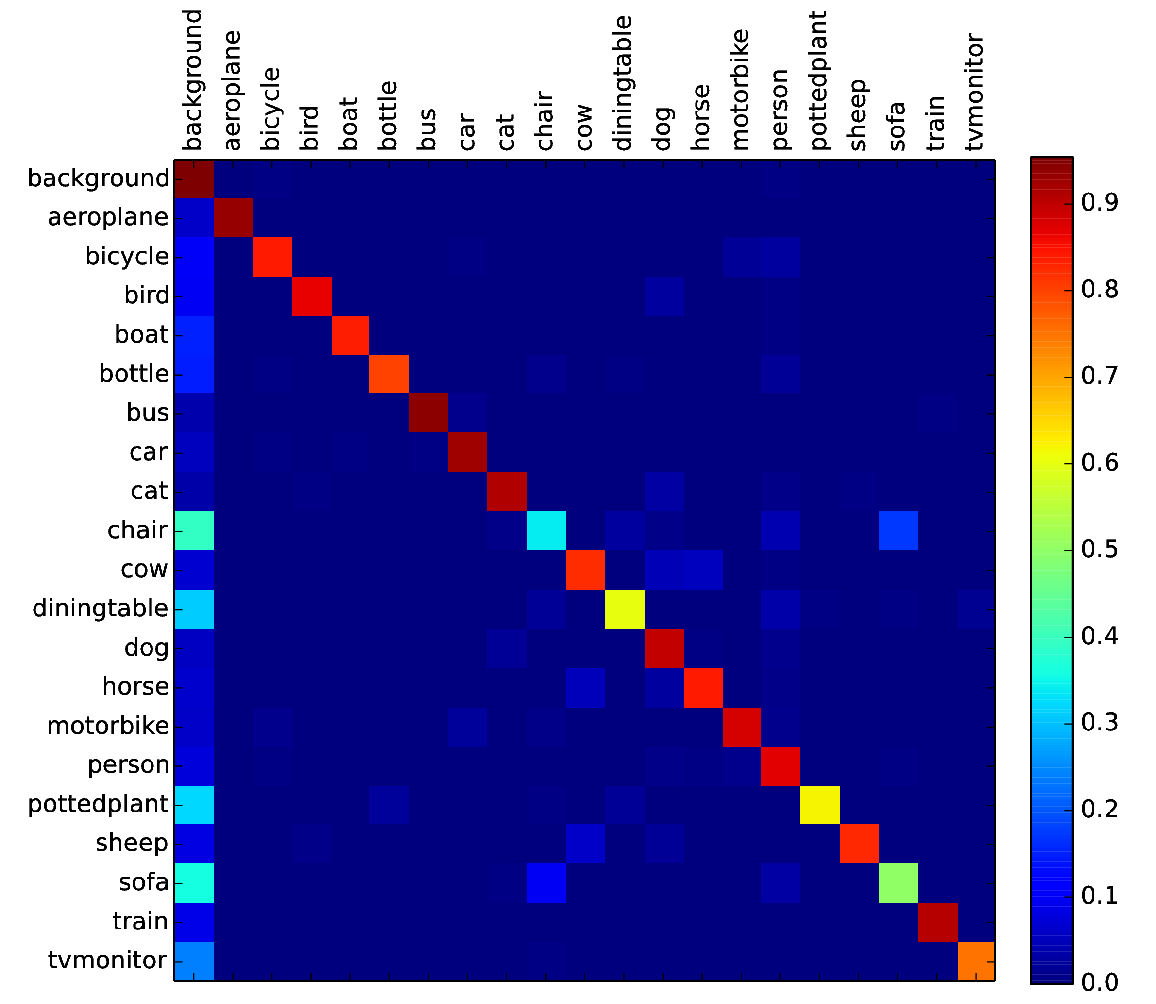
\includegraphics[width=0.5\textwidth]{confusion.pdf}
  \caption{图号、图题置于图的下方}
%  \bicaption{图号、图题置于图的下方}{Sample figure 1}
  \label{fig:confusion}
  \figurenote{若有图注,图注置于图题下方。
    多个图注则须顺序编号,注序左缩进2字,与注文之间空一字符,续行悬挂缩进左对齐,两端对齐。
    注文的字数较少且是短语时,末尾不可加标点,多个图注可以在同一行通过自由选取字符空格将各个图注间隔开来;
    注文的字数较多或者甚至需要用句子说明时,该图注可以独立成行。
  }
\end{figure}

关于图片的并排,推荐使用较新的 \pkg{subcaption} 宏包,
不建议使用 \pkg{subfigure} 或 \pkg{subfig} 等宏包。



\section{算法环境}

模板中使用 \pkg{algorithm2e} 宏包实现算法环境。关于该宏包的具体用法,
请阅读宏包的官方文档。

\begin{algorithm}
  \SetAlgoLined
  \KwData{this text}
  \KwResult{how to write algorithm with \LaTeX2e }

  initialization\;
  \While{not at end of this document}{
    read current\;
    \eIf{understand}{
      go to next section\;
      current section becomes this one\;
    }{
      go back to the beginning of current section\;
    }
  }
  \caption{算法示例1}
  \label{algo:algorithm1}
\end{algorithm}

注意,我们可以在论文中插入算法,但是插入大段的代码是愚蠢的。
然而这并不妨碍有的同学选择这么做,对于这些同学,建议用 \pkg{listings} 宏包。
